%% % $Id: delete.tex 10922 2010-04-21 11:26:09Z alexandra $
%% % Local Variables:
%% % ispell-check-comments: nil
%% % Local IspellDict: american
%% % End:
%% % --------------------------------------------------------
%% % User documentation
%% % copyright by BREDEX GmbH 2005
%% % --------------------------------------------------------
%% % this command can be inserted multiple times
%% \gdhelpid{}
%% % 
%% \begin{bxdescription}
%% \end{bxdescription}
%% %
%% \begin{bxsteps}
%% % use the \item command for single steps
%% \end{bxsteps}
%% % change <FILE> to the same filename you are editing
%% \bxinput{Links/<FILE>}
%% %
%% % other usefull commands are
%% %   \bxhint{}        to create a hint
%% %   \bxwarn{}        to describe a warning
\index{Project!Delete}
\index{Delete Project}
\begin{enumerate}
\item To delete a \gdproject{} from the database, select:\\
\bxmenu{Test}{Delete}{}.
\item If you haven't already logged into the \gddb{}, a dialog will appear to ask you to do so.  See the previous section \bxpref{tasksdblogin} for details. 
\item Choose the \gdproject{} you want to delete from the combo box in the dialog (\bxfigref{deleteproject}).
 \begin{figure}[h]
\begin{center}
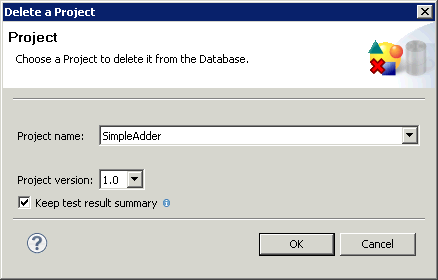
\includegraphics{Tasks/Projects/PS/deleteproject}
\caption{Delete \gdproject{} dialog}
\label{deleteproject}
\end{center}
\end{figure}

\item If there is more than one version of the \gdproject{}, choose which version you want to delete. 
\item Select whether you want to keep the test result summaries associated with this \gdproject{} or not. 
\bxtipp{In productive databases where you wish to evaluate test results over longer periods of time, we recommend selecting the option to keep the summaries.}
\item Click \bxcaption{OK} to delete the selected \gdproject{}. 
\item Confirm the deletion in the dialog which appears.
\bxwarn{Deleting a \gdproject{} from the \gddb{} cannot be undone!}
\end{enumerate}
